\section*{Assignment 04: Monetisation Strategy}
\addcontentsline{toc}{section}{Assignment 04: Monetisation Strategy}

This section distils our messy spreadsheets into a plan for how SkillSync earns money without suffocating the still-fragile network effects.

\subsection*{Revenue streams on the table}
\begin{itemize}
  \item \textbf{Completion fee on each project.} Organisations pay 7\% of the stipend once both sides mark the project successful, keeping monetisation tied to the value we orchestrate while staying invisible to students \citep{HagiuWright2013}.
  \item \textbf{Enablement subscription.} Larger NGOs and public agencies can upgrade to a 499~DKK/month Partner tier that unlocks templated briefs, analytics, and a dedicated coach, mirroring \citet{Choudary2016}'s push for producer tools.
  \item \textbf{Talent insights add-on.} When we have enough data we sell aggregated skill trends to universities and municipal innovation units, guarded by differential privacy and explicit consent so we do not trigger the surveillance trap \citet{Zuboff2019} warns about.
  \item \textbf{Grant-backed scholarships.} Social-impact grants subsidise student stipends for NGOs who cannot afford the fee so inclusion improves while subsidies still accelerate network effects \citep{ShapiroVarian1999}.
\end{itemize}

\subsection*{Timing across the platform lifecycle}
I anchor the roadmap in the classic seed $\rightarrow$ grow $\rightarrow$ harvest logic \citep{Choudary2016}.
\begin{enumerate}
  \item \textbf{Seeding (0--6 months).} No fees yet; we sign memoranda of understanding, chase 30 completed projects, and focus on trust rituals such as office hours and templated retrospectives.
  \item \textbf{Early growth (months 7--12).} Introduce the 7\% completion fee for new organisations while grandfathering the original cohort for three months, pilot the Partner tier with five agencies, and track completion above 85\% plus churn below 10\%.
  \item \textbf{Mature growth (beyond month 12).} Scale the fee to everyone, roll out the Partner tier broadly, launch the insights add-on, and track revenue per active organisation alongside NPS and tool adoption so monetisation deepens engagement.
\end{enumerate}

\subsection*{Experiments and guardrails}
To stay honest we run three experiments: an A/B test on when organisations see the completion fee, Van Westendorp pricing interviews to validate the Partner tier before hard-coding 499~DKK, and a 15-person diary study on whether insights reporting feels empowering or creepy so we can adjust consent flows \citep{Reillier2017}. Each experiment has a rollback plan parked in Notion.

We also mapped the cost side so top-line revenue does not fool us. Fixed year-one spend sits around 620,000~DKK (two builders plus design and hosting) and variable costs track finished projects via payment processing, mentor stipends, and support time. Under conservative assumptions we break even at roughly 1,050 projects per year, matching the activation roadmap in Assignment~09 and heeding \citet{ShapiroVarian1999}'s reminder to know your cost curves.

Figure~\ref{fig:student-profile} puts a face on monetisation. The upgraded student profile surfaces badges, skill heatmaps, and endorsement timelines---the producer tools NGOs buy because they compress due diligence into a glance. Students gain from the ``next skill to showcase'' nudge powered by our data network effect, and the refreshed `Student-Profile.png` proves the thesis rests on real feature bundles, not abstract spreadsheets.

\begin{figure}[h]
  \centering
  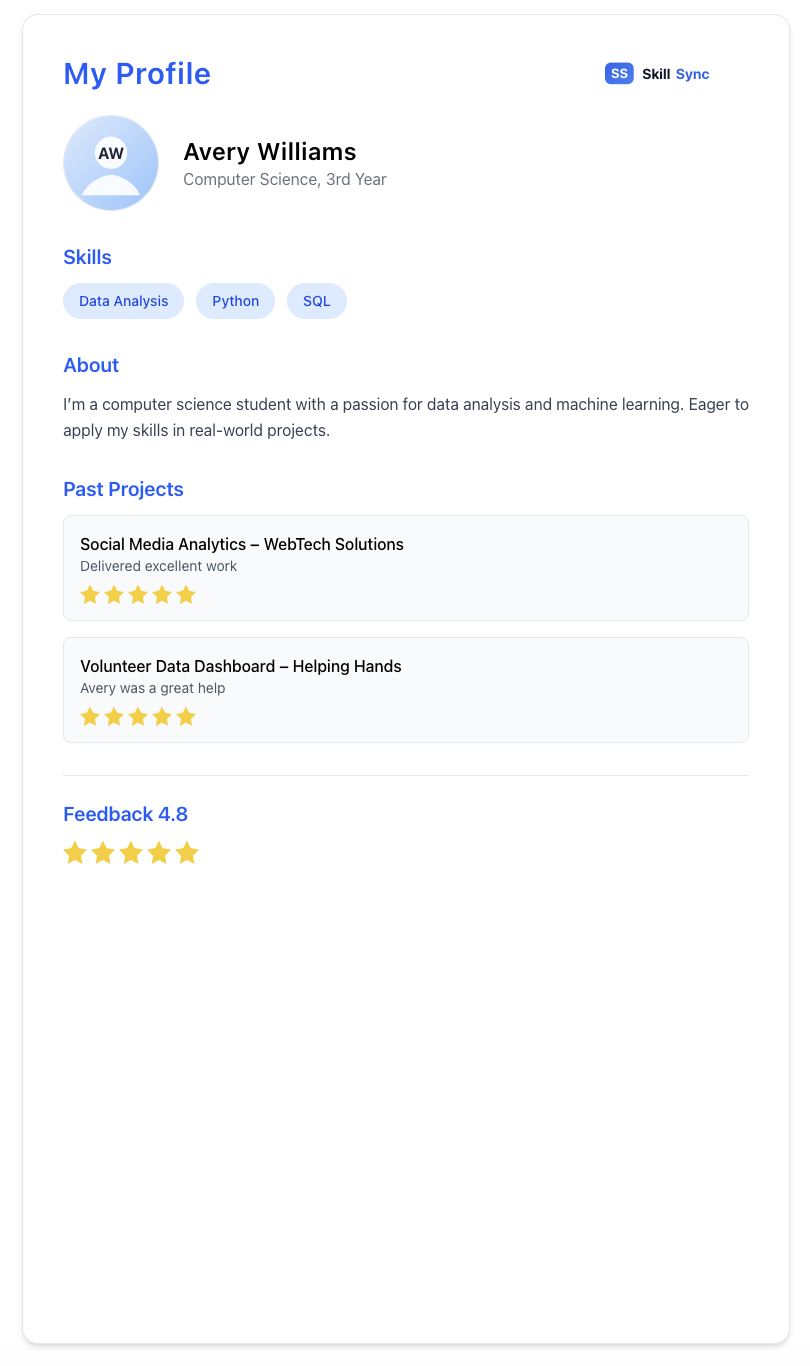
\includegraphics[width=0.8\linewidth]{Student-Profile.png}
  \caption{Student profile (`Student-Profile.png`).}
  \label{fig:student-profile}
\end{figure}

Finally, we pressure-test ethical boundaries. The insights add-on only ships after five organisations in a sector and 500 projects so deanonymisation risk stays low; consent flows spell out ``why we collect this'' and offer easy opt-outs. Grants stay separate from transaction fees so subsidies never distort price signals, honouring the warnings from \citet{Zuboff2019} and \citet{Srnicek2017}.
